\section{Evaluation} \label{sec:Evaluation}

In this section we evaluate our key-value store and the B+-Tree library. The following experiments were ran on a 13-inch early 2015 Macbook Pro\footnote{Processor: 2.7 GHz Intel Core i5. RAM: 8GB}.

\subsection{B+-Tree Experiments}

In this section we evaluate the following claims that our B+-Tree library: 
\begin{itemize}
    \item provides amortized constant time sequential (put or get) operation.
    \item benefits from performance improvements when a sequence of (put or get) operations is partially sorted by key.
\end{itemize}

To evaluate the performance of B+-Tree get operations, we timed how long it took to move to / get all the keys in a B+-Tree for different workloads. That is, we visited or retrieved all the keys in the B+-Tree sequentially, in partially-sorted order and randomly for different B+-Tree sizes. There are three types of partially sorted workloads: those sorted in batches of 15 key-value pairs (\textit{PS Batches 15}), workloads with 1000 sorted batches each with size N / 1000 (\textit{PS Batches N / 1000}) and, finally, workloads with 100 sorted batches each with size N / 100 (\textit{PS Batches N / 100}).  For each B+-Tree with size $N$, the B+-Tree was constructed by inserting all the keys from $0$ to $N - 1$. The results of this experiment are shown in Figure \ref{fig:B+GetsGraph}. 


\begin{figure}[hbtp]
    \centering
    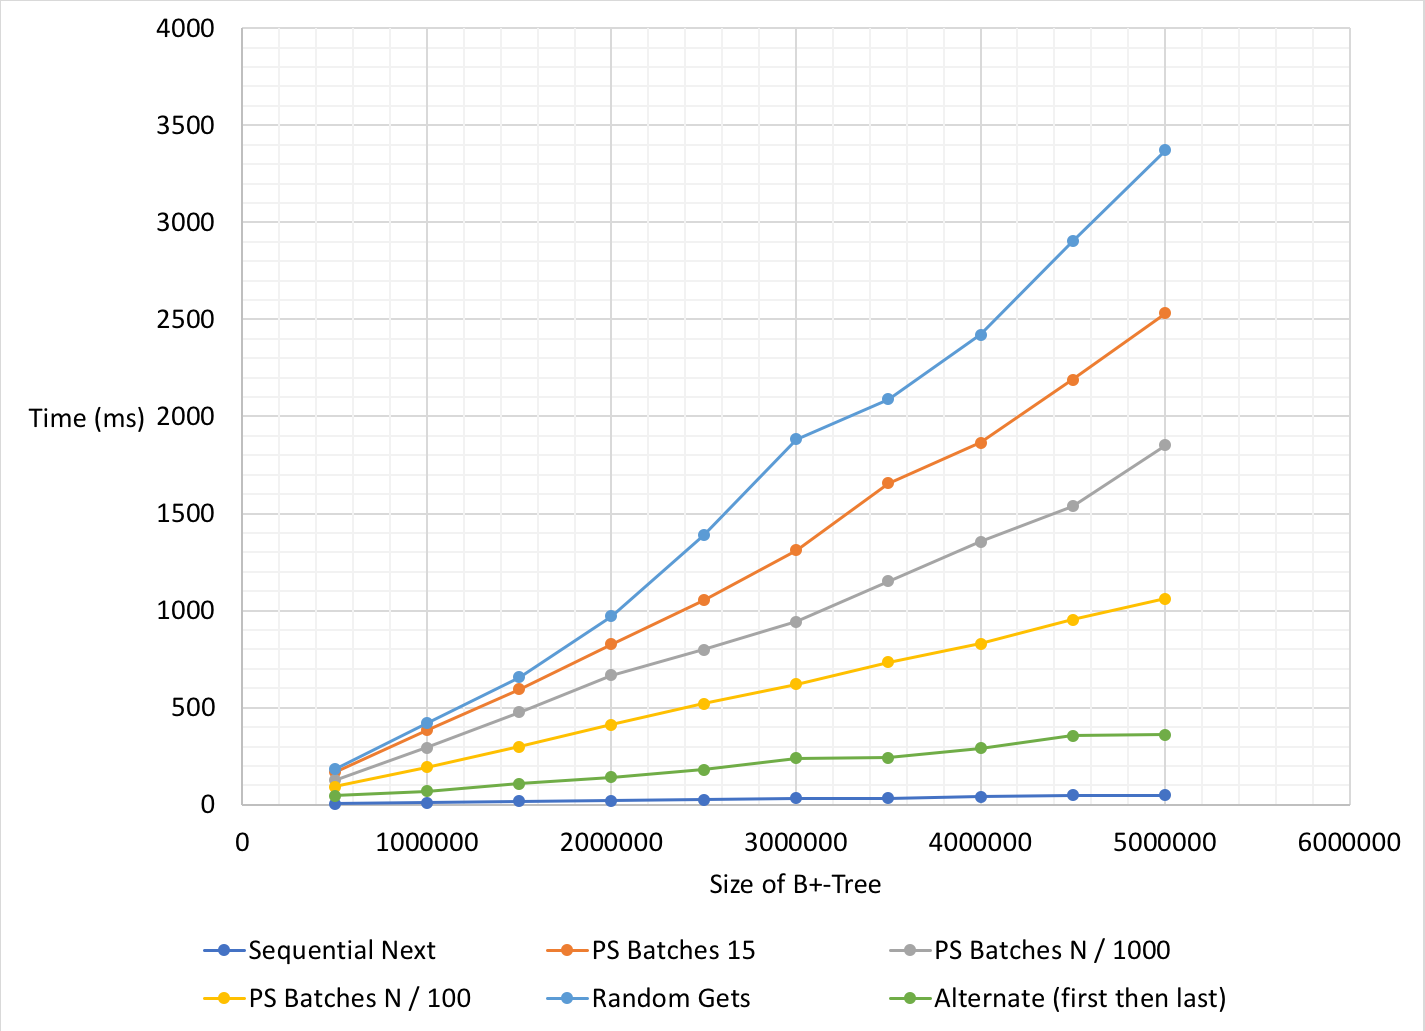
\includegraphics[scale=0.50]{figures/Btreegetsgraph.png}
    \caption{Time to visit or get all the keys in a B+-Tree for different B+-Tree sizes and different workloads.}
    \label{fig:B+GetsGraph}
\end{figure}

Similarly to evaluate the performance of B+-Tree put operations, we timed how long it took to insert a sequence of keys into the B+-Tree with the aforementioned workloads (sequential, partially-sorted and random). Results are shown in Figure \ref{fig:B+PutsGraph} Finally, we use the doubling hypothesis \cite{sedgewick2011algorithms} to empirically measure the order of growth of sequential and random operations . The doubling hypothesis states that if $T(N) \sim aN^blgN$ then $\frac{T(2N)}{T(N)} \sim 2^b$. So by calculating the log ratios of the times taken, we can estimate the order of growth of our B+-Tree under different workloads. 




\begin{figure}[htbp]
    \centering
    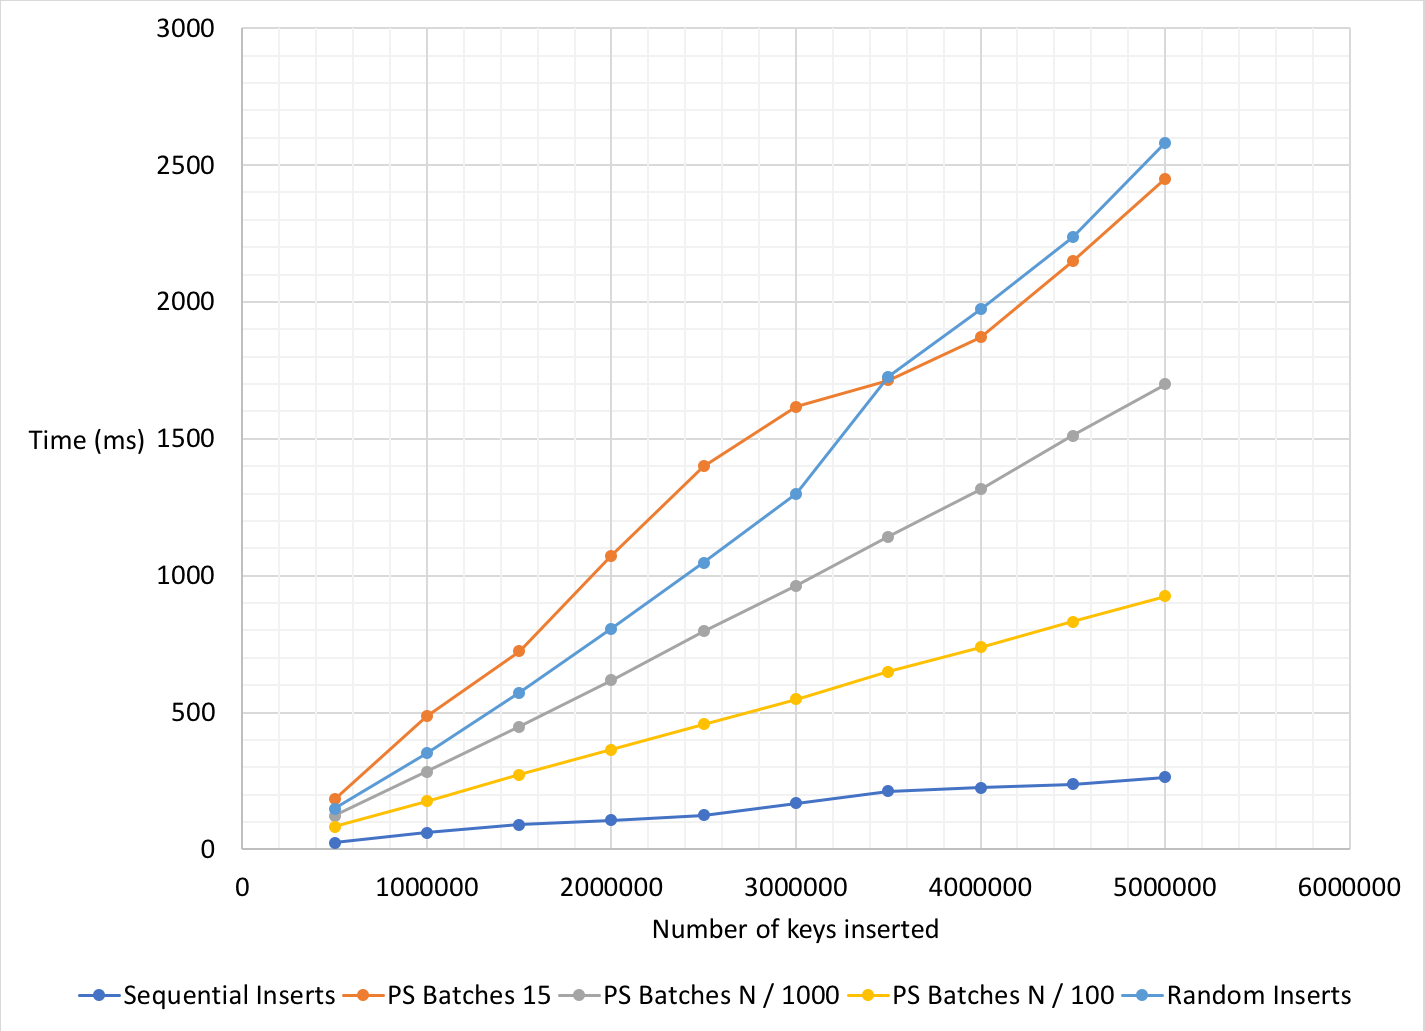
\includegraphics[scale=0.50]{figures/Btreeinsertsgraph.png}
    \caption{Time to insert all keys from 0 to size - 1 into an empty B+-Tree for different sizes and different workloads.}
    \label{fig:B+PutsGraph}
\end{figure}


As we can see from Figures \ref{fig:B+GetsGraph} and \ref{fig:B+PutsGraph} sequential operations are very fast inx our B+-Tree, while random operations are the slowest. We also see that our B+-Trees have performance gains if a series of put or get operations are partially sorted into sorted batches. The larger the sorted batches are in proportion to the number of keys to be inserted or retrieved, the larger the performance gain. On a different note, we expected that alternately retrieving the first and last keys in the B+-Tree its size number of times would model the worst case performance, as each retrieval costs $2 \times height$ node accesses. Even though this should, in theory, model the B+-Tree's worst case behavior it does not in practice, because of caching. If the same two keys are constantly retrieved, the same same ancestor nodes are traversed each time to get from one key to the other. These nodes will be in higher levels of cache memory thereby keeping the cost of node accesses to retrieve each key very low. This experiment highlights the value of cache-friendly data structures when implementing main-memory databases and also highlights how costly main-memory look-ups can be in comparison to cache look-ups.


\begin{figure}[htbp]
    \centering
    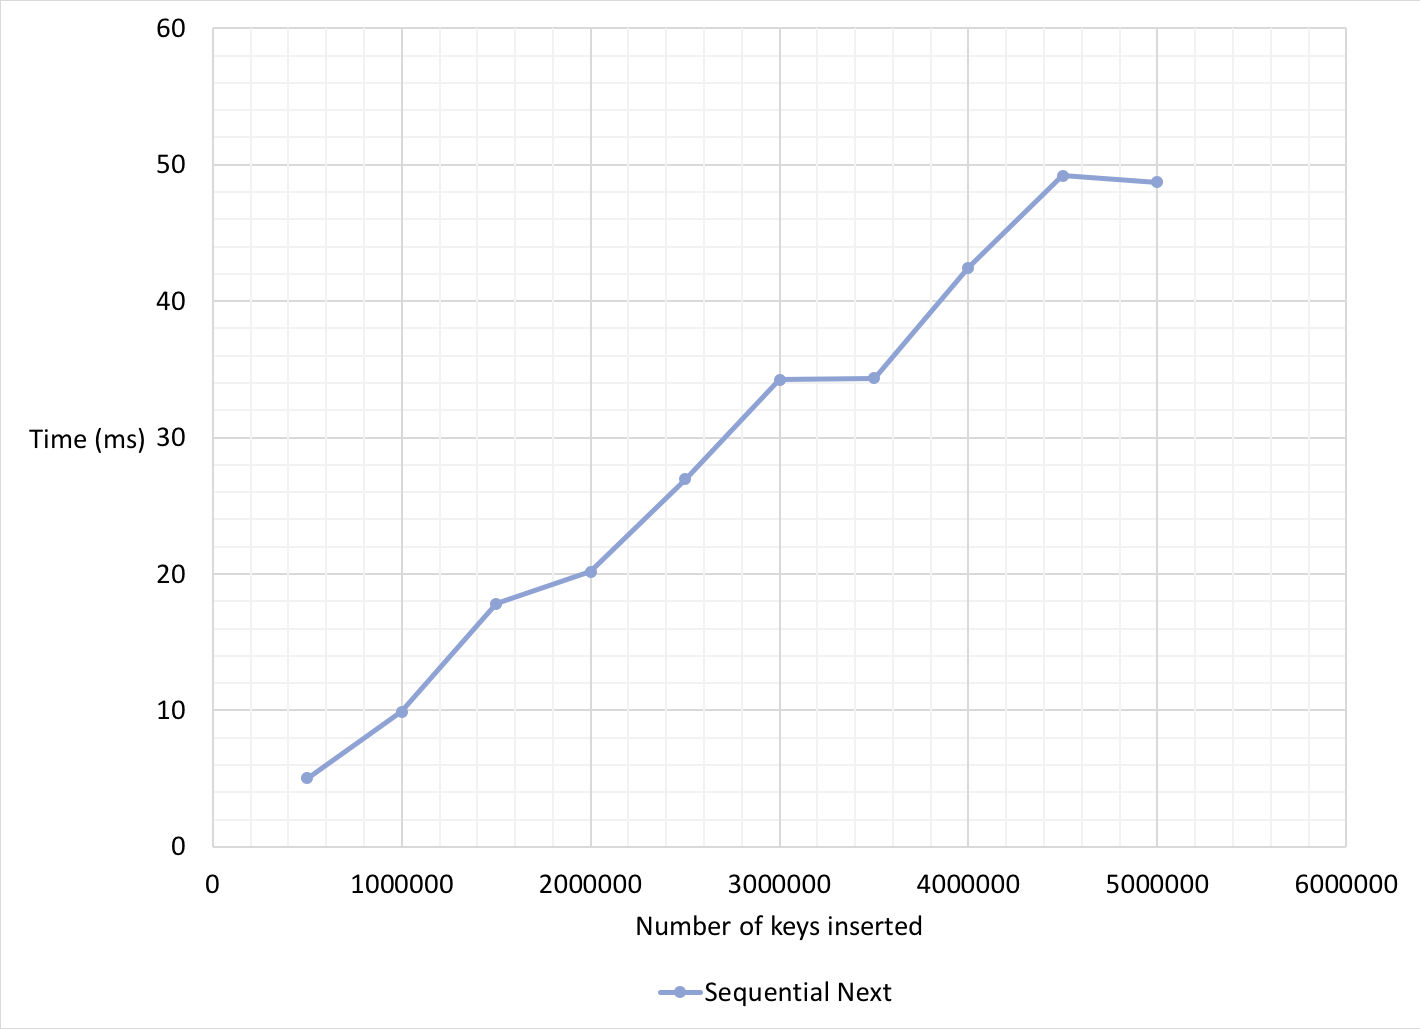
\includegraphics[scale=0.50]{figures/BtreeSequentialNextGraph.png}
    \caption{Time to sequentially visit all the keys in a B+-Tree for different B+-Tree sizes}
    \label{fig:B+GetsSequentialGraph}
\end{figure}

\begin{figure}[htbp]
    \centering
    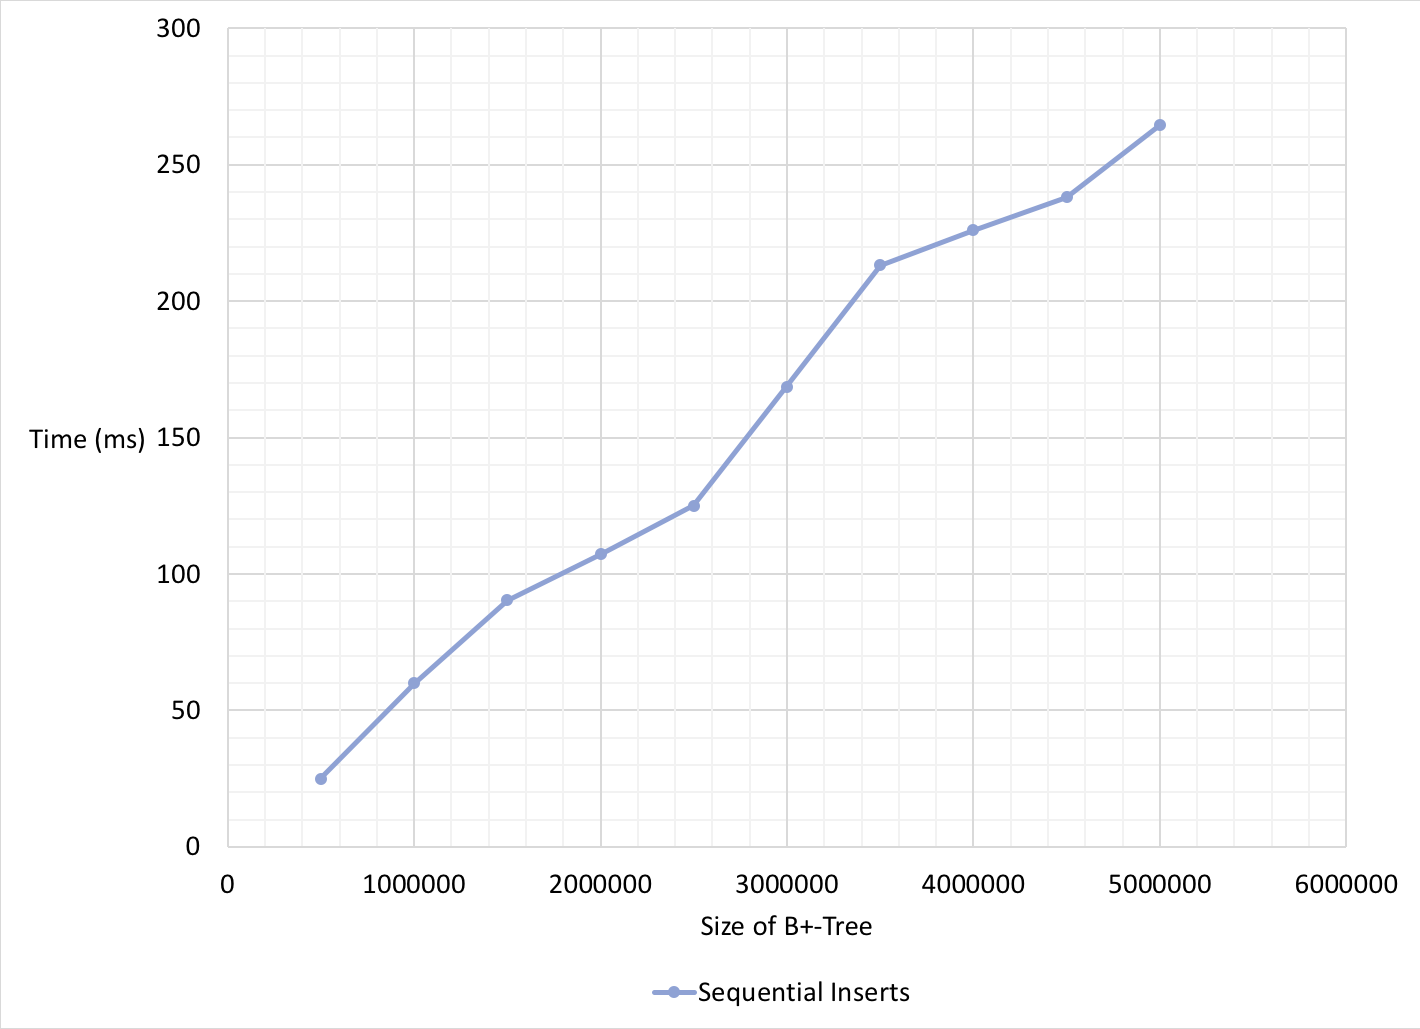
\includegraphics[scale=0.50]{figures/BtreeSequentialnsertsGraph.png}
    \caption{Time to sequentially insert all the keys from 0 to size - 1 into an empty B+-Tree}
    \label{fig:B+PutsSequentialGraph}
\end{figure}

Figures \ref{fig:B+GetsSequentialGraph} and \ref{fig:B+PutsSequentialGraph} allow us to better appreciate the speed of sequential operations. Our B+-Tree implementation can sequentially retrieve all keys from a B+-Tree of size 5 million in about 49 milliseconds; this is about 9.8 nanoseconds per next operation. We can sequentially insert 5 million keys into a B+-Tree in about 265 milliseconds; this is about 53 nanoseconds per next operation. 

\begin{table}[hbtp]
\centering
\label{fig:logRatioGetAnalysis}
\begin{tabular}{|c|c|c|c|c|}
\hline
\multirow{2}{*}{Number of keys (millions)} & \multicolumn{2}{c|}{Move to Next} & \multicolumn{2}{c|}{Random Get} \\ \cline{2-5} 
                                           & Time (ms)       & log ratio       & Time (ms)      & log ratio      \\ \hline
0.5                                        & 5.03            &                 & 182.48         &                \\ \hline
1                                          & 9.89            & 0.975           & 420.07         & 1.203          \\ \hline
2                                          & 20.16           & 1.027           & 970.84         & 1.209          \\ \hline
4                                          & 42.45           & 1.074           & 2421.73        & 1.319          \\ \hline
\end{tabular}
\caption{Log ratio of running times of sequential and random get operations for different key sizes.}
\end{table}

\begin{table}[htbp]
\centering
\label{fig:logRatioPutAnalysis}
\begin{tabular}{|c|c|c|c|c|}
\hline
\multirow{2}{*}{Number of keys (millions)} & \multicolumn{2}{c|}{Sequential Put} & \multicolumn{2}{c|}{Random Put} \\ \cline{2-5} 
                                           & Time (ms)       & log ratio       & Time (ms)      & log ratio      \\ \hline
0.5                                        & 25.01           &                 & 148.83         &                \\ \hline
1                                          & 59.89           & 1.260           & 350.62         & 1.236          \\ \hline
2                                          & 107.29          & 0.841           & 805.68         & 1.200          \\ \hline
4                                          & 225.94          & 1.074           & 1973.40        & 1.292          \\ \hline
\end{tabular}
\caption{Log ratio of running times of sequential and random put operations for different key sizes.}
\end{table}

Using the doubling hypothesis we see that the time complexity of $N$ sequential put or get operations is effectively linear (see see \ref{fig:logRatioGetAnalysis} and \ref{fig:logRatioPutAnalysis}). The log ratio converges to approximately one. However for random operations, even though the log ratio rounds down to 1, the fractional portion hints at an extra logarithmic term. This is in line with our expectation that $N$ random put or get operations is linearithmic.


\subsection{KVStore Experiments}

In this section we evaluate the following claims that our key-value store library: 
\begin{itemize}
    \item performs well when its keys have long common prefixes
    \item benefits from performance improvements when a sequence of operations is partially sorted by key.
\end{itemize}


\begin{figure}[h]
    \centering
    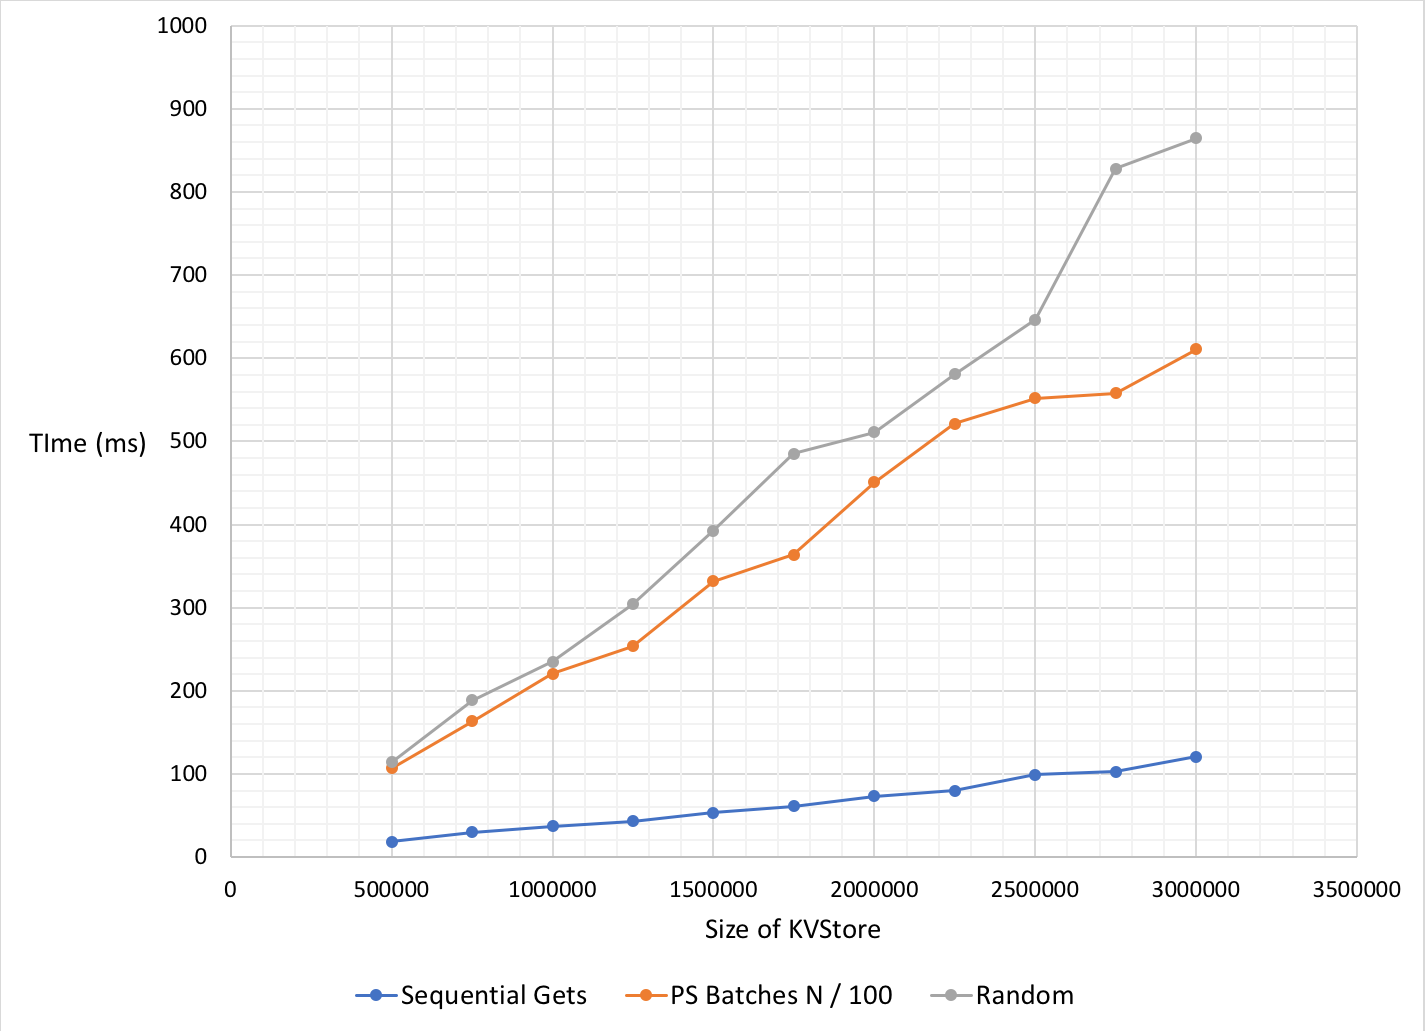
\includegraphics[scale=0.50]{figures/KVStoregetsgraph.png}
    \caption{Time to get all the keys in a KVStore for different sizes and different workloads. Keys are 30 bytes long and are not forced to have common prefixes. Keys are randomly generated.}
    \label{fig:KVStoreGetsGraph}
\end{figure}

Similarly to the B+-Tree experiments we evaluated how long it takes to retrieve all the keys in a KVStore object for different sizes and workloads, where each KVStore object is built with random keys. The results are in \ref{fig:KVStoreGetsGraph}. We see that, as expected sequential gets are very fast. We also see that partially sorting query keys gives performance gains over random query keys. However, the performance gains form partially sorting are not as large as one might expect. There could be different reasons for this. A possibility is that even if the next key being inserted or retrieved is different from the previous key on only the last few bytes, our current KVStore implementation still traverses the trie of B+-Trees from the first layer to the appropriate layer where the keys diverge. Even though we can skip all the layers where the key slices of the next key are the same as the previous key's key slices.


\begin{figure}[h]
    \centering
    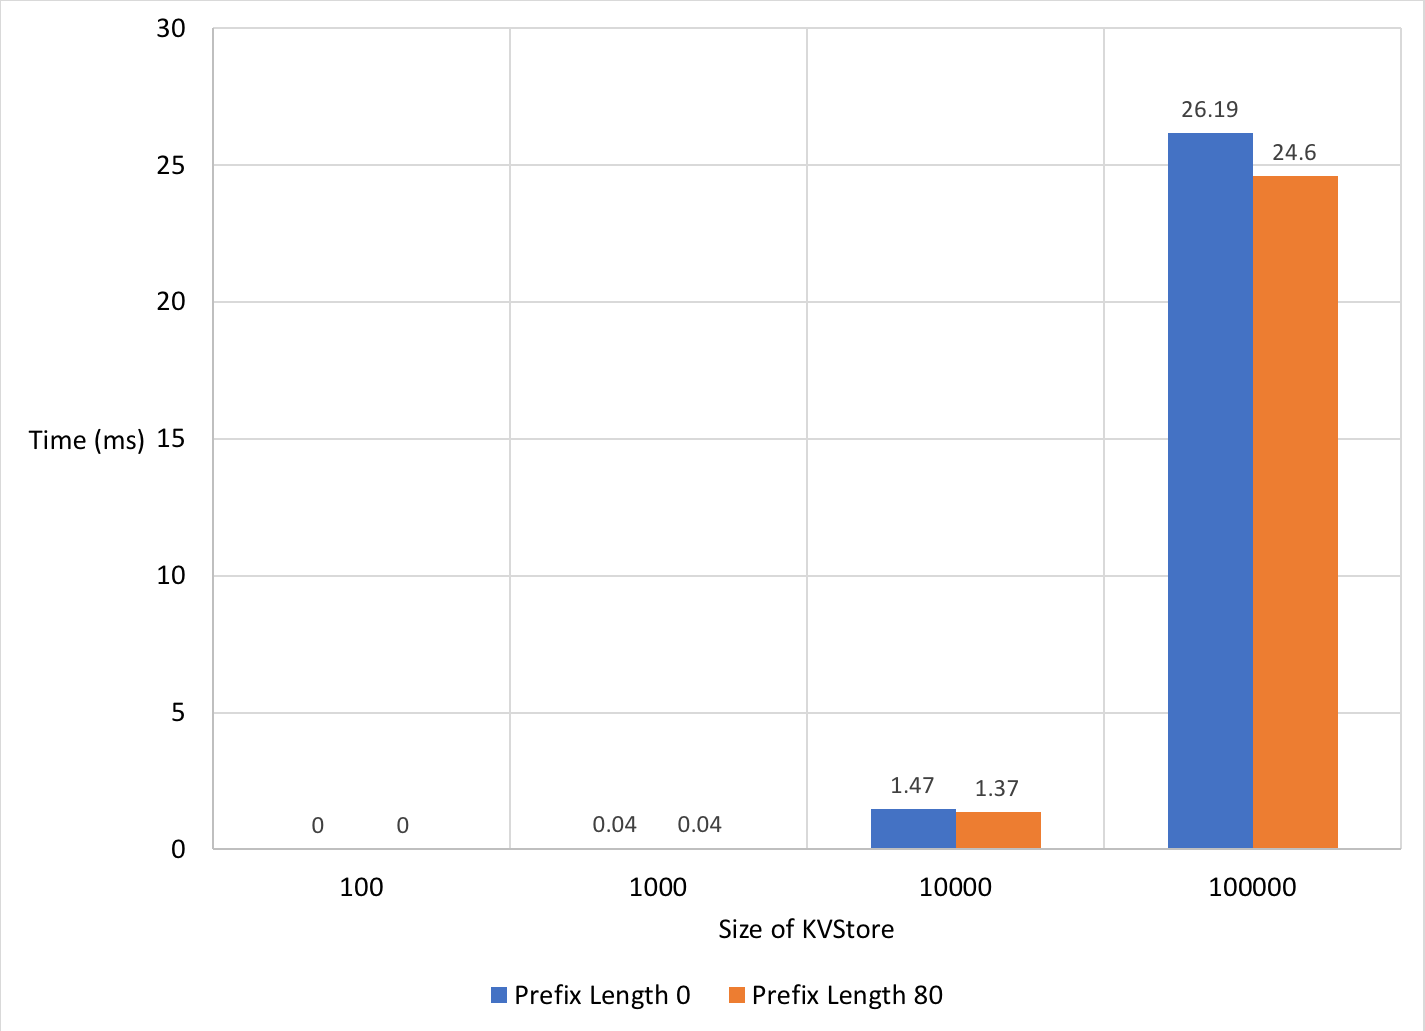
\includegraphics[scale=0.50]{figures/kvstoreprefixgraph.png}
    \caption{Time to get all the keys in a KVStore for different sizes for different common prefix lengths. Keys are 100 bytes long. We compare the behavior of get operations when the first 80 bytes are the same and the remaining 20 bytes are random versus when all 100 bytes are random. Keys are randomly generated.}
    \label{fig:KVStoreCommonPrefixes}
\end{figure}

From our discussion in section \ref{sec:VarLCPKeysMasstree}, the expectation is that a typical B+-Tree implementation and, by extension, a key-value store built from this B+-Tree would suffer performance degradation when most of its keys have long common prefixes. However, our KVStore implementation properly handles this scenario as shown in Figure \ref{fig:KVStoreCommonPrefixes}.In fact our KVStore does slightly better for keys with long common prefixes. This is probably because the first few layers of the KVStore consists of only two nodes each (a B+-Tree leaf node with one entry and a bordernode). Consequently, to get to any key all the nodes containing the common prefix must be visited and so these nodes will be in higher levels of cache memory.
